\documentclass{hessothesis}

\ThesisTitle{APDL : Acquire Process Description Language}
\Author{Sylvain Julmy}
\Supervisor{Pierre-André Mudry}
\SupervisorResearchUnit{Institut Systèmes Industriels}
\ExternalExpert{??}
\ExternalExpertResearchUnit{??}
\Place{Lausanne}
\Date{\today}
\AuthorEmail{sylvain.julmy@gmail.com}
\Orientation{Information and Communication Technologies (ICT)}

\bibliography{bibliography.bib}

\newacronym{IoT}{IoT}{Internet of Things}
\newacronym{DSL}{DSL}{Domain specific language}
\newacronym{VDSML}{VDSML}{Visual Domain Specific Modeling Language}
\newacronym{APDL}{APDL}{Acquire and Process Description Language}

%%% Local Variables:
%%% mode: latex
%%% TeX-master: "thesis"
%%% End:


\begin{document}

\maketitle

\makeinfopage

\part{Introduction}
\label{part:introduction}

\newChapter{Introduction}{cha:introduction}

The \gls{IoT} is one of the most prolific domains in computer science
nowadays. There are connected objects everywhere and the amount of data that we
receive from them is growing day after day. Everybody wants to measure some
environment variables using a simple and cheap device like an Arduino or a
Raspberry Pi.

On another hand, people who want to use those devices are often not familiar
with the hardware and/or the software parts of an IoT project. For example, a
chemistry engineer could be interested to measure some values in the air, but he
is absolutely not in the IoT domain.

\section{Context}
\label{sec:intro-context}

Imagine an electrical engineer who needs to create a system which is able to
recover data from multiple sensors, like external temperature and barometric
pressure. With that data, the engineer needs to compute a new pressure value
with the temperature and compare it to the one given by the barometric pressure
sensor using graph plot.

The problem for this electrical engineer is the software part. He doesn't know how
to send data through the network, recover them and store them into a database
for a future plot. On another hand, a software engineer would not know the hardware part.

IoT programming is at some point a merge of some specific domains like Software,
Hardware, Telecommunication and Design. The figure \ref{fig:basic_archi} illustrates
this concept of multi-domain project. Are involved in this concept:

\begin{itemize}
\item Hardware.
\item Software.
\item Design.
\item Telecommunication.
\end{itemize}

\begin{figure}[H]
  \centering
  \fbox{
    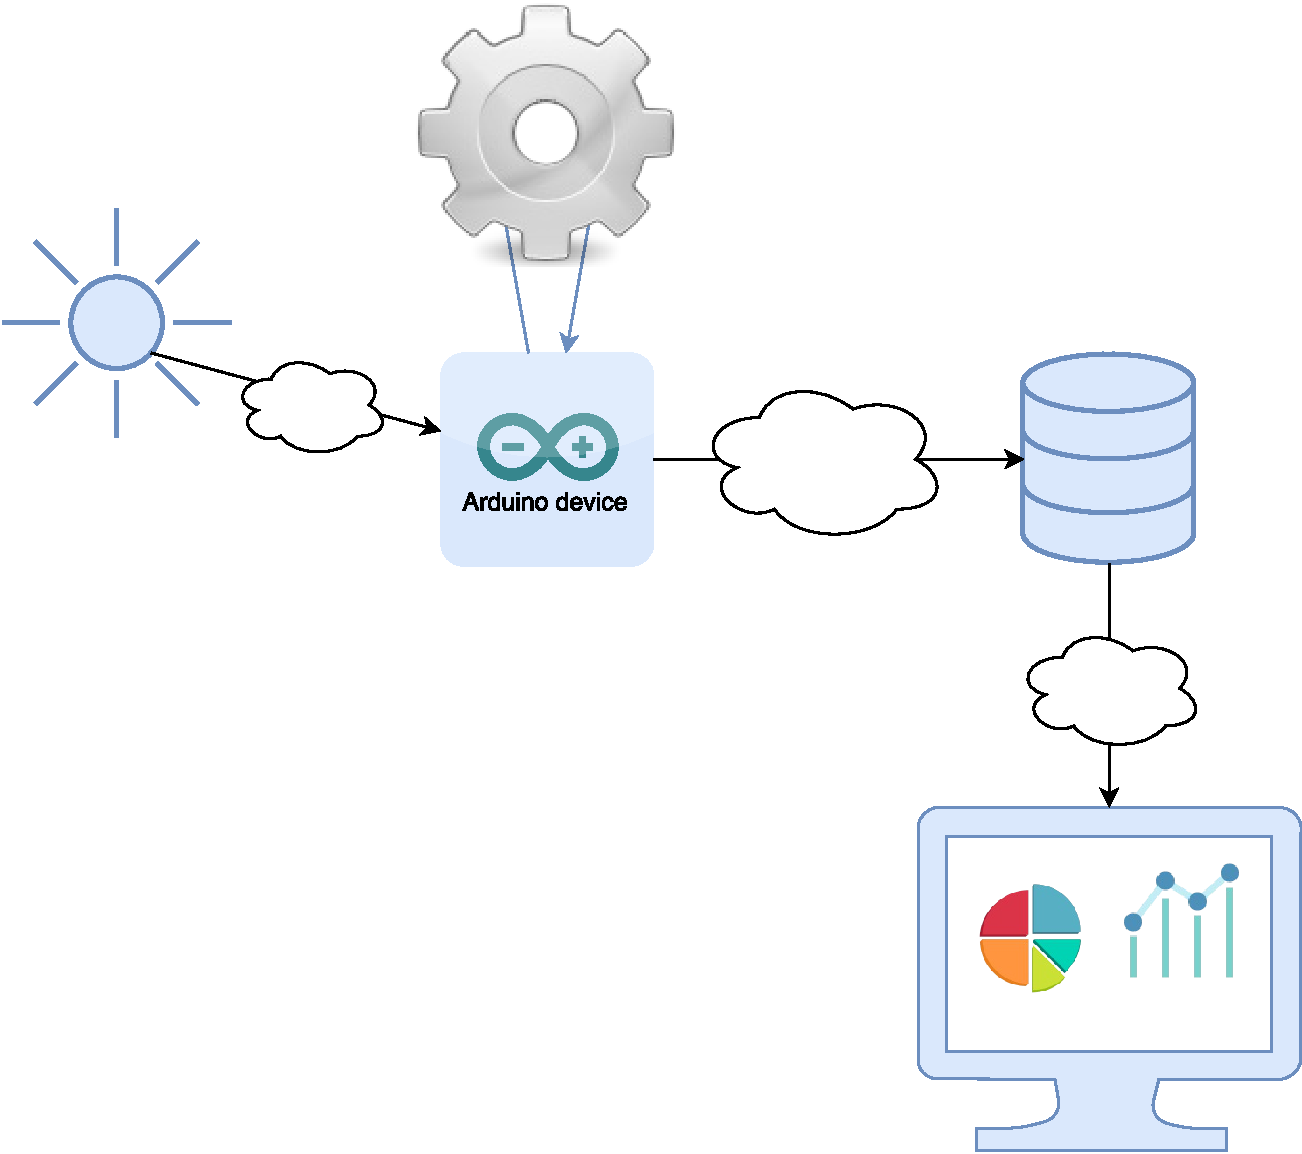
\includegraphics[width=0.4\textwidth]{img/basic_archi}
    }
  \caption[Basic APDL architecture example]{ Visualisation of the involved domains
in the APDL ecosystem : hardware, software, design and
telecommunication. And sometimes, a person doesn't know any part of this.}
  \label{fig:basic_archi}
\end{figure}

\section{Problem Statement}
\label{sec:intro-problem-statement}

According to the previous example we could say that not everybody could develop
a project like this from scratch. Maybe some people have the whole knowledge to
do this by themselves but not a lambda person.

The major issue with such project is the people diversity. Bringing together people from various
professions creates several difficulties : team management, various programming knowledge, different
project's perception, and many more.

\section{Solution Statement}
\label{sec:intro-solution-statement}

The \gls{APDL} ecosystem goal is to
provide a simple way to describe such a pipeline. From the sampling of the data
from a sensor and its transformation to the display of the result of charts through
storing them into a database or send them to a specific server.

\section{Outline of this thesis}
\label{sec:intro-roadmap}

We have set ourselves the challenge of providing a simple way to design specific
\gls{IoT} projects. Before setting out to tackle it, we firstly look at the state
of the art in \gls{DSL} development and \gls{IoT} challenges. Some work has
been done in the field of Domain specific frameworks and languages for \gls{IoT}.

The main technical chapters includes chapter~\ref{chap:dsl_design},
\ref{chap:dsl_implementation}, \ref{chap:dsl_validation}. In
chapter~\ref{chap:dsl_design}, we present the design of the \gls{APDL}
\gls{DSL}. We set out the domain of interest and explore the development process
of the language. Chapter \ref{chap:dsl_implementation} presents the
implementation of the designed language and illustrates the compilation process
used by \gls{APDL}. In chapter \ref{chap:dsl_validation} we present the
validation of the implemented compiler and the generated output based on a set
of APDL programs designed for this purpose. We also mention a testing
technique called property-based testing which has simplified the parser tests.
Finally, in chapter~\ref{chap:apdl_ecosystem}, we present the work done about
the APDL ecosystem and its utilisation through an example realised from scratch.

%%% Local Variables:
%%% mode: latex
%%% TeX-master: "../thesis"
%%% End:


\part{A Domain specific language for the Internet of Things}
\label{part:dsl}

\chapter{State of the art}

IoT is a huge area of research and development over the few past year,
developer and researcher in this field face some serious challenge
\cite{DBLP:conf/mipro/2015}\cite{Gubbi20131645}\cite{bendickson2016}:

\begin{itemize}
\item Device diversity (Arduino, Raspberry PI, physical sensors, biometric
sensors)
\item Software implementation (Linux, iOS, Windows, Android)
\item Interactive modes (publisher/subscriber pattern, request/response
pattern, command pattern, pull/push pattern)
\item Engineering unit (degree Farenheit/degree Celsius, foot/metre, and
many more)
\item Power management and optimisation
\item Connectivity, the device is connected with various protocols like ZigBee
or MQTT
\item Reliability, the device could be instantly checked and have some error
handling application level
\item Data description, we need to annotate the produced data (raw data are a problem)
\item Various security problems:
  \begin{itemize}
  \item Physical security
  \item Data exchange security
  \item Cloud storage security
  \item Update and patch
  \end{itemize}
\end{itemize}

In this part, a state of the art and some various approaches for the
IOT programming, development and design are presented. We will see some
programming language which one could be the target of the DSL we are creating
and some existing domain specific language. In the end, we fully describe the
challenge of the IOT in order to offer a language which is able to answer all
the developers wishes.

\section{Programming Language for the Internet of Things}
\label{sec:proglang-for-iot}

Using a programming language to create IOT Applications offer full control to
the developer, but it comes to the handling of the challenge too. By the way, some
language needs to embed interpreter and/or virtual machine in order to work. This
adds some additional memory, power and processor use.

\subsection{C/C++}
\label{subsec:cc++}

C and C++ are available for compilation on almost every platform, it’s a
hardware focused language which is not too complex and offers great speed and
memory management. The very big advantages is that C and C++ are compiled, they
don’t need a runtime management and compiled binaries are very small for limited
memory devices. From another point of view, the programmer needs to do almost
everything by itself: memory management, pointer arithmetic error handling
and, if we use C, there is no standard library for data structure and algorithm.

Notice that the Arduino language is a subset of C and owns the same advantages
and problems with memory management.

Therefore, C and C++ are really good when it comes to a small device with very
little memory and when no operating system are available.

\subsection{Python}
\label{subsec:python}

Python is a programming language created in 1990 by Guido van Rossum, it’s an
object-oriented, imperative and interpreted one. Because Python is interpreted,
the language needs to run with a virtual machine.

By the way, a tool named Cython\cite{behnel2010cython} is able to compile, after
some work, a Python code to a C executable, which removes the interpreter and
virtual machine needed at the origin.

We can go further, some embedded system for IOT does not run an operating system
(the Arduino for example) and Cython need to have access to some operating
system features. But there is some work about the possibility to run Python
without any OS\cite{jakeedge2015}.

On the other hand, Python owns a great community with tons of tutorials and library
for the IOT programming and especially with the Raspberry PI.

\subsection{Java}
\label{subsec:java}

C and C++ are great programming language for the IOT, it becomes easier to manage
and control the hardware with that language, but they are hardware specific
too. We can’t write a program and run it into every possible hardware. Maybe a
device is running on Linux and another one is running on Windows. The probably
best answer to this problem is Java\cite{Waher:2015:LIT:2789499}, which supports
multiple hardware design through his virtual machine if the IOT project run
needs to run on different platforms.

\subsection{Another Programming Languages}
\label{subsec:other-prog-lang}

There are many programming languages available for IOT development, we don’t want
to describe them all but we want a small overview of the field for the
development of the DSL. We could talk a lot about language like Go, Rust and
Javascript, which could be very good for a specific part of an IOT project.

We don’t need to know all the usable programming language for the IOT, but we
need a target for our DSL and those languages advantages and disadvantages
would be considering for further work.

\section{Domain specific language for the Internet of Things}
\label{sec:dsl-for-iot}

Research and work has been done during the past year on the domain specific
language for the Internet of Things. Programming for the IOT could be really
anoying for the software developer who are not familliar with the hardware oriented
concept or for the electrical enginner which are not software oriented. We need
to know both soft and hard part of the project in order to realise it.

We present an overview of some research and technologies around the DSL created
for the IOT. Notice that when the DSL is a visual one, we call it a VDSML :
Visual Domain Specific Modeling Language.

\subsection{Node-red}
\label{subsec:node-red}

Node-red\cite{node-red} is a tool, develop with Node.js and browser focused, for
wiring the internet of things together. It is a purely VDSML without, practicly,
no code to write. Node-red has compatibility with a lot of popular platforms\cite{node-red} :
\begin{itemize}
\item Raspberry Pi
\item BeagleBone Black
\item Android
\item Arduino
\item Docker
\item Amazon AWS
\item IBM Bluemix
\item Microsoft Azure
\end{itemize}

But we can go further, Node-red provides an editor, builtin function, a full
compatibility with Javascript and the Node.js packages and finally a way to save
and share graph information of the project with JSON.

Node-red is capable of simply create a complete pipeline from our diagram with
just a mouse click. Using block for programming and connect some basic features
do not require a high knowledge level.

\subsubsection{Example}
\label{subsub:node-red-example}

\subsection{DSL-4-IoT}
\label{subsec:dsl-4-iot}

\subsection{DiaSuite}
\label{subsec:diasuite}

\subsection{PervML}
\label{subsec:pervml}

\subsection{OpenHab}
\label{subsec:openhab}

\subsection{LogicIOT}
\label{subsec:logic-iot}

\subsection{ArduinoML}
\label{subsec:arduino-ml}

\section{Internet of Things programming challenge}
\label{sec:iot-prog-challenge}

Power supply, power-optimized algorithm, network protocols

Dynamic power management (DPM), to shud down device when they don’t need to be
online

DPM --> problem because of the latency and latency is an overall problem

Reliability: device could be constantely checked and Error handling procedure
in the application level

Data curation and data brokering: device could produce a huge ammount of data

Data projection

Data description: metadata to describe raw-data

Declarative programming for the IOT !!!

%%% Local Variables:
%%% mode: latex
%%% TeX-master: "../thesis"
%%% End:
\chapter{A Domain specific language}
\label{cha:a-dsl}

A Domain specific language \gls{Dsl} is a programming language whose the goal is
to provide a way to solve specific domain problem. For example, Matlab is a
domain specific language because, in the first place, it was for matrix
manipulation and mathematic.

What we call ``domain'' is a set of problem related together in the same scope.
For Matlab, those domain could be a matrix multiplication or the resolution of a
equantion system. Those to operation are related to numerical mathematic and
that is the ``domain'' of Matlab.

This chapter will introduce and discuss the question ``Why use a DSL ?'' by
exposing some advantages that \gls{APDL} could bring for non-IoT-developers.
Then we present the diffenrence between an internal and an external DSL and the
advantages and disadvantages for both of them. Then we will conclude this
chapter by exposing the development phase of a DSL describe by Van Deursen and
Klint \cite{little_languages_little_maintenance}.

\section{Why use a Dsl ?}
\label{sec:why-use-dsl}

\section{Internal Dsl vs. External Dsl}
\label{sec:dsl-internal-vs-external}

\section{Advantages and Disadvantages of a Dsl}
\label{sec:dsl-advantages-disadvantages}

\section{Dsl Development phases}
\label{sec:dsl-dev-phases}

%%% Local Variables:
%%% mode: latex
%%% TeX-master: "../thesis"
%%% End:

\chapter{Design of the DSL}
\label{cha:dsl-design}

As mentionned by Van Deursen and Klint
\cite{little_languages_little_maintenance}, one point is to cluster the
knowledge we acquire into a set of semantic notions and opertions on them. This
chapter will present the whole design of the APDL DSL. Firstly, we analyse all
the concept we need to have for a complete DSL design for our case-study. Those
concept include the data source, the transmission, the storage and finally the
visualisation of the data.

Then, we will present the design of the library which is implementing the
clustered information.

\section{Data source}
\label{sec:dsl-design-data-source}

The concept of data source include some different information :
\begin{itemize}
\item The source device
\item The type of data
\item The sampling
\end{itemize}

\subsection{Source device}
\label{subsec:dsl-design-source-device}

Firstly, we have to know that there is a lot of different existing device for
the IoT programming, some of them are just connected ones like bluethoot tracker
or smart device like fridge or door. For the purpose of the project we are just
going the take device that are sensor oriented. All we want is to gather
information for the environmment and communicate it to whatever we want.

TODO : write about arduino and raspeberry

%%% Local Variables:
%%% mode: latex
%%% TeX-master: "../thesis"
%%% End:

\chapter{Implementation}
\label{cha:dsl_implementation}

%%% Local Variables:
%%% mode: latex
%%% TeX-master: "../thesis"
%%% End:

\chapter{Test}
\label{cha:dsl_test}

%%% Local Variables:
%%% mode: latex
%%% TeX-master: "../thesis"
%%% End:


\printbibliography

\printglossaries

% \listoftables
% \listoffigures
% \listoflistings

\end{document}

%%% Local Variables:
%%% TeX-command-extra-options: "-shell-escape"
%%% mode: latex
%%% TeX-master: t
%%% End: